\chapter{Literature Review} \label{chap:lit-review}

The purpose of this literature review is to explain the context
for the research directions for this project. This section also
provides background knowledge specific to the silent speech
domain which should help familiarise readers with this particularly
niche subject area.

\section{Key Terms}

A list of silent speech and speech recognition domain specific key terms are provided
to familiarise the reader with certain concepts to help the reader digest this report.

\begin{itemize}
\item \emph{Word Error Rate (WER):}
Metric used in speech recognition systems which accounts for differences in length of
a recognised word sequence and a reference word sequence. WER is derived from
Levenshtein distance  which is a string metric for measuring the difference between two
sequences. The Levenshtein distance between two words is essentially the minimum number of
single-character edits (including insertions, deletions or substitutions) required to
change one word into another. Another term for it is the "edit distance".
\[
  WER
  = \dfrac{S + D + I}{N}
  = \dfrac{S + D + I}{S + D + C}
\]
Where each term means:\\
S: Number of substitutions\\
D: Number of deletions\\
I: Number of insertions\\
C: Number of correct words\\
N: Number of words in the reference (N = S+D+C)
(\cite{1966SPhD...10..707L})
\item \emph{Mel-Spectrogram:}
A mel spectrogram 
\end{itemize}

\section{Digital Voicing of Silent Speech}

There are two primary landmark papers released in the silent speech domain
which this project takes large inspiration from. These are
"Digital Voicing of Silent Speech" (\cite{gaddy2020digital}) and
"An Improved Model for Voicing Silent Speech" (\cite{gaddy2021improved}).

\subsection{Relevance}

As the primary goal of my project was to find new methods of improving silent
speech systems in general, it was useful to find an open-source silent speech
dataset which could either be used for producing audio speech from silent
speech or classifying silent speech into text.

\section{Data Augmentation via EMG Synthesis}

\subsection{Data Augmentation Background}

Data augmentation refers to techniques which are used to either increase
the amount of available training data by adding slightly modified
copies of the original data or to synthesize new examples entirely.
The purpose of this is to regularise the training and help reduce overfitting
when training a machine learning model (\cite{data_augmentation_def}).

Many methods exist to generate augmented data for machine learning.
One of them is to apply geometric transformations such as: translations, rotations,
cropping, flipping, scaling, etc. (\cite{data_augmentation_def}).

This method is commonly applied in the computer vision domain and
leads to substantial improvements in performance. For instance,
when cropping was applied to an image recognition dataset for the
Caltech 101 dataset, it lead to a Top-1 score increase of 13.82\%
(\cite{geometric_augment}).

\subsection{Applicability to EMG Domain}

However unlike images, EMG data is a collection of non-stationary
time-series data which has been collected from different electrodes
and also contains many other artefacts such as baseline noise,
powerline interference and other contamination (\cite{semg_filtering}).
Moreover, simple geometric transformations are not necessarily appropriate
for EMG as they may impact time domain features as EMG signals are
1-dimensional.

Further to this, in computer vision projects, it is easy to determine whether
an augmented dataset is similar to the original signal. However for EMG
signals, it is difficult to determine if an augmented dataset has still
retained key properties of the original dataset.
Figure \ref{fig:real-vs-pred-emg} provides a sample of an original
EMG data recording during vocalised speech and the synthesized EMG
data, for an utterance from this project to demonstrate this difficulty.
Although both of the data samples appear similar, when they are used in
a transduction model to produce speech, they sound noticably different from
each other because of the difference within the smaller time windows.

\begin{figure}[hbtp]
    \caption{Original vs Synthesized Vocal EMG Data from EMG Synthesis Approach}
    \label{fig:real-vs-pred-emg}
    \centering
    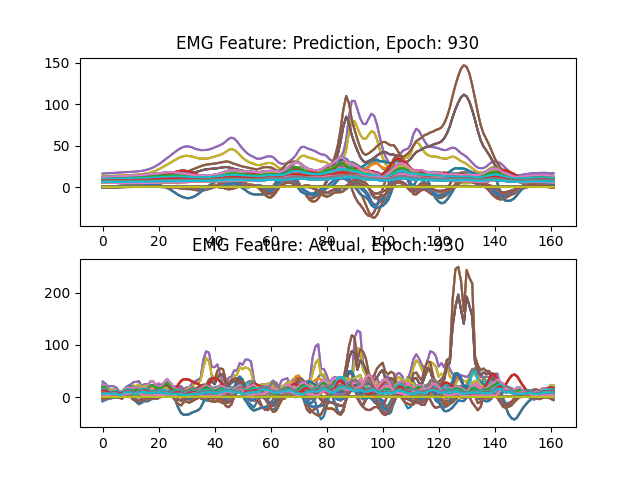
\includegraphics[width=0.75\linewidth]{graphics/emg_augment/real_vs_synth.png}
\end{figure}

\subsection{Successful EMG Augmentation Approaches}

Despite this, there have been many successful data augmentation techniques
for EMG and simliar EEG signals.